% SOURCE: edit-harness/results/merging/Llama-3.2-1B_L12_RG/RG_operating_curve_table.json fields model; layer; per_g_summary[*].qualifies; verdict.overall
% SOURCE: edit-harness/results/merging/Llama-3.1-8B_L24_RG/RG_operating_curve_table.json fields model; layer; per_g_summary[*].qualifies; verdict.overall
% SOURCE: edit-harness/results/merging/Mistral-7B-v0.3_L24_RG/RG_operating_curve_table.json fields model; layer; per_g_summary[*].qualifies; verdict.overall
% SOURCE: edit-harness/results/merging/Qwen2.5-1.5B_L21_RG/RG_operating_curve_table.json fields model; layer; per_g_summary[*].qualifies; verdict.overall
% SOURCE: edit-harness/results/merging/Qwen2.5-7B_L21_RG/RG_operating_curve_table.json fields model; layer; per_g_summary[*].qualifies; verdict.overall
% SOURCE: edit-harness/results/merging/Qwen2.5-14B_L36_RG/RG_operating_curve_table.json fields model; layer; per_g_summary[*].qualifies; verdict.overall
% DERIVATION: boundary=max(integer g where per_g_summary[g].qualifies==true); INCONCLUSIVE maps to undefined, never zero.
% SCOPE: all selected cells are 75% relative depth; model width and edited layer remain distinct fields; no within-model depth curve is plotted.
% !TEX encoding = UTF-8 Unicode
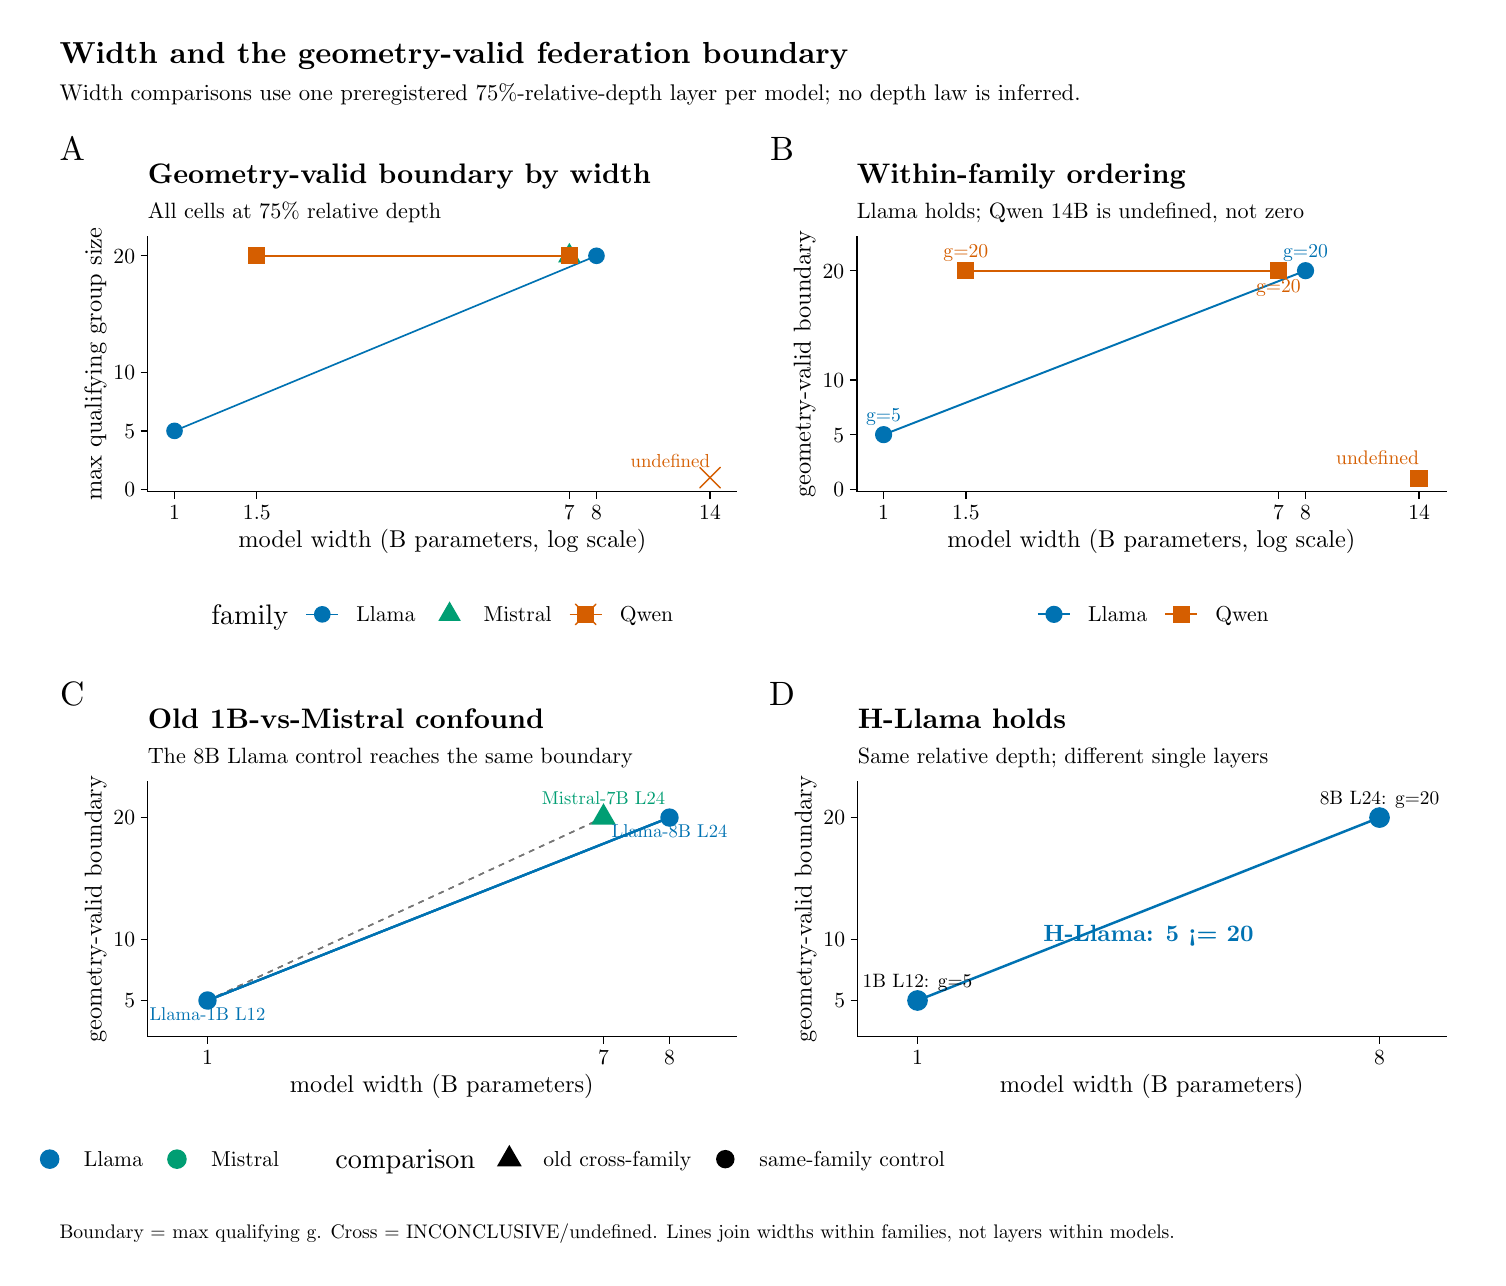
\begin{tikzpicture}[x=1pt,y=1pt]
\definecolor{fillColor}{RGB}{255,255,255}
\path[use as bounding box,fill=fillColor,fill opacity=0.00] (0,0) rectangle (523.96,444.46);
\begin{scope}
\path[clip] (  0.00,  0.00) rectangle (523.96,444.46);
\definecolor{drawColor}{RGB}{255,255,255}
\definecolor{fillColor}{RGB}{255,255,255}

\path[draw=drawColor,line width= 0.6pt,line join=round,line cap=round,fill=fillColor] (  0.00,  0.00) rectangle (523.96,444.46);
\end{scope}
\begin{scope}
\path[clip] (  5.50,214.13) rectangle (262.23,410.99);
\definecolor{drawColor}{RGB}{255,255,255}
\definecolor{fillColor}{RGB}{255,255,255}

\path[draw=drawColor,line width= 0.5pt,line join=round,line cap=round,fill=fillColor] (  5.50,214.13) rectangle (262.23,410.99);
\end{scope}
\begin{scope}
\path[clip] (262.23,214.13) rectangle (518.46,410.99);
\definecolor{drawColor}{RGB}{255,255,255}
\definecolor{fillColor}{RGB}{255,255,255}

\path[draw=drawColor,line width= 0.5pt,line join=round,line cap=round,fill=fillColor] (262.23,214.13) rectangle (518.46,410.99);
\end{scope}
\begin{scope}
\path[clip] ( 43.39,276.78) rectangle (256.23,368.89);
\definecolor{fillColor}{RGB}{255,255,255}

\path[fill=fillColor] ( 43.39,276.78) rectangle (256.23,368.89);
\definecolor{drawColor}{RGB}{0,114,178}

\path[draw=drawColor,line width= 0.6pt,line join=round] ( 53.06,298.76) --
	(205.53,362.02);
\definecolor{drawColor}{RGB}{213,94,0}

\path[draw=drawColor,line width= 0.6pt,line join=round] ( 82.79,362.02) --
	(195.74,362.02);
\definecolor{fillColor}{RGB}{0,114,178}

\path[fill=fillColor] ( 53.06,298.76) circle (  3.01);

\path[fill=fillColor] (205.53,362.02) circle (  3.01);
\definecolor{fillColor}{RGB}{0,158,115}

\path[fill=fillColor] (195.74,366.70) --
	(199.79,359.68) --
	(191.69,359.68) --
	cycle;
\definecolor{fillColor}{RGB}{213,94,0}

\path[fill=fillColor] ( 79.78,359.01) --
	( 85.80,359.01) --
	( 85.80,365.03) --
	( 79.78,365.03) --
	cycle;

\path[fill=fillColor] (192.73,359.01) --
	(198.74,359.01) --
	(198.74,365.03) --
	(192.73,365.03) --
	cycle;

\path[draw=drawColor,line width= 0.5pt,line join=round,line cap=round] (242.85,278.18) -- (250.27,285.60);

\path[draw=drawColor,line width= 0.5pt,line join=round,line cap=round] (242.85,285.60) -- (250.27,278.18);

\node[text=drawColor,anchor=base east,inner sep=0pt, outer sep=0pt, scale=  0.68] at (246.56,285.44) {undefined};
\end{scope}
\begin{scope}
\path[clip] (  0.00,  0.00) rectangle (523.96,444.46);
\definecolor{drawColor}{RGB}{0,0,0}

\path[draw=drawColor,line width= 0.5pt,line join=round,line cap=rect] ( 43.39,276.78) --
	( 43.39,368.89);
\end{scope}
\begin{scope}
\path[clip] (  0.00,  0.00) rectangle (523.96,444.46);
\definecolor{drawColor}{RGB}{0,0,0}

\node[text=drawColor,anchor=base east,inner sep=0pt, outer sep=0pt, scale=  0.78] at ( 38.80,274.98) {0};

\node[text=drawColor,anchor=base east,inner sep=0pt, outer sep=0pt, scale=  0.78] at ( 38.80,296.07) {5};

\node[text=drawColor,anchor=base east,inner sep=0pt, outer sep=0pt, scale=  0.78] at ( 38.80,317.16) {10};

\node[text=drawColor,anchor=base east,inner sep=0pt, outer sep=0pt, scale=  0.78] at ( 38.80,359.33) {20};
\end{scope}
\begin{scope}
\path[clip] (  0.00,  0.00) rectangle (523.96,444.46);
\definecolor{drawColor}{RGB}{0,0,0}

\path[draw=drawColor,line width= 0.5pt,line join=round] ( 40.84,277.67) --
	( 43.39,277.67);

\path[draw=drawColor,line width= 0.5pt,line join=round] ( 40.84,298.76) --
	( 43.39,298.76);

\path[draw=drawColor,line width= 0.5pt,line join=round] ( 40.84,319.84) --
	( 43.39,319.84);

\path[draw=drawColor,line width= 0.5pt,line join=round] ( 40.84,362.02) --
	( 43.39,362.02);
\end{scope}
\begin{scope}
\path[clip] (  0.00,  0.00) rectangle (523.96,444.46);
\definecolor{drawColor}{RGB}{0,0,0}

\path[draw=drawColor,line width= 0.5pt,line join=round,line cap=rect] ( 43.39,276.78) --
	(256.23,276.78);
\end{scope}
\begin{scope}
\path[clip] (  0.00,  0.00) rectangle (523.96,444.46);
\definecolor{drawColor}{RGB}{0,0,0}

\path[draw=drawColor,line width= 0.5pt,line join=round] ( 53.06,274.23) --
	( 53.06,276.78);

\path[draw=drawColor,line width= 0.5pt,line join=round] ( 82.79,274.23) --
	( 82.79,276.78);

\path[draw=drawColor,line width= 0.5pt,line join=round] (195.74,274.23) --
	(195.74,276.78);

\path[draw=drawColor,line width= 0.5pt,line join=round] (205.53,274.23) --
	(205.53,276.78);

\path[draw=drawColor,line width= 0.5pt,line join=round] (246.56,274.23) --
	(246.56,276.78);
\end{scope}
\begin{scope}
\path[clip] (  0.00,  0.00) rectangle (523.96,444.46);
\definecolor{drawColor}{RGB}{0,0,0}

\node[text=drawColor,anchor=base,inner sep=0pt, outer sep=0pt, scale=  0.78] at ( 53.06,266.82) {1};

\node[text=drawColor,anchor=base,inner sep=0pt, outer sep=0pt, scale=  0.78] at ( 82.79,266.82) {1.5};

\node[text=drawColor,anchor=base,inner sep=0pt, outer sep=0pt, scale=  0.78] at (195.74,266.82) {7};

\node[text=drawColor,anchor=base,inner sep=0pt, outer sep=0pt, scale=  0.78] at (205.53,266.82) {8};

\node[text=drawColor,anchor=base,inner sep=0pt, outer sep=0pt, scale=  0.78] at (246.56,266.82) {14};
\end{scope}
\begin{scope}
\path[clip] (  0.00,  0.00) rectangle (523.96,444.46);
\definecolor{drawColor}{RGB}{0,0,0}

\node[text=drawColor,anchor=base,inner sep=0pt, outer sep=0pt, scale=  0.88] at (149.81,256.69) {model width (B parameters, log scale)};
\end{scope}
\begin{scope}
\path[clip] (  0.00,  0.00) rectangle (523.96,444.46);
\definecolor{drawColor}{RGB}{0,0,0}

\node[text=drawColor,rotate= 90.00,anchor=base,inner sep=0pt, outer sep=0pt, scale=  0.88] at ( 26.74,322.84) {max qualifying group size};
\end{scope}
\begin{scope}
\path[clip] (  0.00,  0.00) rectangle (523.96,444.46);
\definecolor{fillColor}{RGB}{255,255,255}

\path[fill=fillColor] ( 61.27,220.13) rectangle (238.35,244.78);
\end{scope}
\begin{scope}
\path[clip] (  0.00,  0.00) rectangle (523.96,444.46);
\definecolor{drawColor}{RGB}{0,0,0}

\node[text=drawColor,anchor=base west,inner sep=0pt, outer sep=0pt, scale=  1.02] at ( 66.37,228.94) {family};
\end{scope}
\begin{scope}
\path[clip] (  0.00,  0.00) rectangle (523.96,444.46);
\definecolor{fillColor}{RGB}{255,255,255}

\path[fill=fillColor] ( 99.23,225.23) rectangle (113.68,239.68);
\definecolor{drawColor}{RGB}{0,114,178}

\path[draw=drawColor,line width= 0.6pt,line join=round] (100.68,232.46) -- (112.24,232.46);
\definecolor{fillColor}{RGB}{0,114,178}

\path[fill=fillColor] (106.46,232.46) circle (  3.01);
\end{scope}
\begin{scope}
\path[clip] (  0.00,  0.00) rectangle (523.96,444.46);
\definecolor{fillColor}{RGB}{255,255,255}

\path[fill=fillColor] (145.22,225.23) rectangle (159.68,239.68);
\definecolor{fillColor}{RGB}{0,158,115}

\path[fill=fillColor] (152.45,237.13) --
	(156.50,230.12) --
	(148.40,230.12) --
	cycle;
\end{scope}
\begin{scope}
\path[clip] (  0.00,  0.00) rectangle (523.96,444.46);
\definecolor{fillColor}{RGB}{255,255,255}

\path[fill=fillColor] (194.42,225.23) rectangle (208.87,239.68);
\definecolor{drawColor}{RGB}{213,94,0}

\path[draw=drawColor,line width= 0.6pt,line join=round] (195.86,232.46) -- (207.43,232.46);
\definecolor{fillColor}{RGB}{213,94,0}

\path[fill=fillColor] (198.64,229.45) --
	(204.65,229.45) --
	(204.65,235.46) --
	(198.64,235.46) --
	cycle;

\path[draw=drawColor,line width= 0.5pt,line join=round,line cap=round] (197.93,228.75) -- (205.36,236.17);

\path[draw=drawColor,line width= 0.5pt,line join=round,line cap=round] (197.93,236.17) -- (205.36,228.75);
\end{scope}
\begin{scope}
\path[clip] (  0.00,  0.00) rectangle (523.96,444.46);
\definecolor{drawColor}{RGB}{0,0,0}

\node[text=drawColor,anchor=base west,inner sep=0pt, outer sep=0pt, scale=  0.78] at (118.78,229.77) {Llama};
\end{scope}
\begin{scope}
\path[clip] (  0.00,  0.00) rectangle (523.96,444.46);
\definecolor{drawColor}{RGB}{0,0,0}

\node[text=drawColor,anchor=base west,inner sep=0pt, outer sep=0pt, scale=  0.78] at (164.78,229.77) {Mistral};
\end{scope}
\begin{scope}
\path[clip] (  0.00,  0.00) rectangle (523.96,444.46);
\definecolor{drawColor}{RGB}{0,0,0}

\node[text=drawColor,anchor=base west,inner sep=0pt, outer sep=0pt, scale=  0.78] at (213.97,229.77) {Qwen};
\end{scope}
\begin{scope}
\path[clip] (  0.00,  0.00) rectangle (523.96,444.46);
\definecolor{drawColor}{RGB}{0,0,0}

\node[text=drawColor,anchor=base west,inner sep=0pt, outer sep=0pt, scale=  0.80] at ( 43.39,375.55) {All cells at 75\% relative depth};
\end{scope}
\begin{scope}
\path[clip] (  0.00,  0.00) rectangle (523.96,444.46);
\definecolor{drawColor}{RGB}{0,0,0}

\node[text=drawColor,anchor=base west,inner sep=0pt, outer sep=0pt, scale=  1.02] at ( 43.39,388.14) {\bfseries Geometry-valid boundary by width};
\end{scope}
\begin{scope}
\path[clip] (  0.00,  0.00) rectangle (523.96,444.46);
\definecolor{drawColor}{RGB}{0,0,0}

\node[text=drawColor,anchor=base,inner sep=0pt, outer sep=0pt, scale=  1.22] at ( 16.09,396.37) {A};
\end{scope}
\begin{scope}
\path[clip] (299.61,276.78) rectangle (512.46,368.89);
\definecolor{fillColor}{RGB}{255,255,255}

\path[fill=fillColor] (299.61,276.78) rectangle (512.46,368.89);
\definecolor{drawColor}{RGB}{0,114,178}

\path[draw=drawColor,line width= 0.7pt,line join=round] (309.29,297.40) --
	(461.75,356.65);
\definecolor{drawColor}{RGB}{213,94,0}

\path[draw=drawColor,line width= 0.7pt,line join=round] (339.01,356.65) --
	(451.96,356.65);
\definecolor{fillColor}{RGB}{0,114,178}

\path[fill=fillColor] (309.29,297.40) circle (  3.11);

\path[fill=fillColor] (461.75,356.65) circle (  3.11);
\definecolor{fillColor}{RGB}{213,94,0}

\path[fill=fillColor] (335.90,353.53) --
	(342.13,353.53) --
	(342.13,359.76) --
	(335.90,359.76) --
	cycle;

\path[fill=fillColor] (448.85,353.53) --
	(455.08,353.53) --
	(455.08,359.76) --
	(448.85,359.76) --
	cycle;

\path[fill=fillColor] (499.67,278.49) --
	(505.90,278.49) --
	(505.90,284.72) --
	(499.67,284.72) --
	cycle;
\definecolor{drawColor}{RGB}{0,114,178}

\node[text=drawColor,anchor=base,inner sep=0pt, outer sep=0pt, scale=  0.71] at (309.29,302.30) {g=5};

\node[text=drawColor,anchor=base,inner sep=0pt, outer sep=0pt, scale=  0.71] at (461.75,361.55) {g=20};
\definecolor{drawColor}{RGB}{213,94,0}

\node[text=drawColor,anchor=base,inner sep=0pt, outer sep=0pt, scale=  0.71] at (339.01,361.55) {g=20};

\node[text=drawColor,anchor=base,inner sep=0pt, outer sep=0pt, scale=  0.71] at (451.96,348.81) {g=20};

\node[text=drawColor,anchor=base east,inner sep=0pt, outer sep=0pt, scale=  0.71] at (502.78,286.50) {undefined};
\end{scope}
\begin{scope}
\path[clip] (  0.00,  0.00) rectangle (523.96,444.46);
\definecolor{drawColor}{RGB}{0,0,0}

\path[draw=drawColor,line width= 0.5pt,line join=round,line cap=rect] (299.61,276.78) --
	(299.61,368.89);
\end{scope}
\begin{scope}
\path[clip] (  0.00,  0.00) rectangle (523.96,444.46);
\definecolor{drawColor}{RGB}{0,0,0}

\node[text=drawColor,anchor=base east,inner sep=0pt, outer sep=0pt, scale=  0.78] at (295.02,274.97) {0};

\node[text=drawColor,anchor=base east,inner sep=0pt, outer sep=0pt, scale=  0.78] at (295.02,294.72) {5};

\node[text=drawColor,anchor=base east,inner sep=0pt, outer sep=0pt, scale=  0.78] at (295.02,314.46) {10};

\node[text=drawColor,anchor=base east,inner sep=0pt, outer sep=0pt, scale=  0.78] at (295.02,353.96) {20};
\end{scope}
\begin{scope}
\path[clip] (  0.00,  0.00) rectangle (523.96,444.46);
\definecolor{drawColor}{RGB}{0,0,0}

\path[draw=drawColor,line width= 0.5pt,line join=round] (297.06,277.65) --
	(299.61,277.65);

\path[draw=drawColor,line width= 0.5pt,line join=round] (297.06,297.40) --
	(299.61,297.40);

\path[draw=drawColor,line width= 0.5pt,line join=round] (297.06,317.15) --
	(299.61,317.15);

\path[draw=drawColor,line width= 0.5pt,line join=round] (297.06,356.65) --
	(299.61,356.65);
\end{scope}
\begin{scope}
\path[clip] (  0.00,  0.00) rectangle (523.96,444.46);
\definecolor{drawColor}{RGB}{0,0,0}

\path[draw=drawColor,line width= 0.5pt,line join=round,line cap=rect] (299.61,276.78) --
	(512.46,276.78);
\end{scope}
\begin{scope}
\path[clip] (  0.00,  0.00) rectangle (523.96,444.46);
\definecolor{drawColor}{RGB}{0,0,0}

\path[draw=drawColor,line width= 0.5pt,line join=round] (309.29,274.23) --
	(309.29,276.78);

\path[draw=drawColor,line width= 0.5pt,line join=round] (339.01,274.23) --
	(339.01,276.78);

\path[draw=drawColor,line width= 0.5pt,line join=round] (451.96,274.23) --
	(451.96,276.78);

\path[draw=drawColor,line width= 0.5pt,line join=round] (461.75,274.23) --
	(461.75,276.78);

\path[draw=drawColor,line width= 0.5pt,line join=round] (502.78,274.23) --
	(502.78,276.78);
\end{scope}
\begin{scope}
\path[clip] (  0.00,  0.00) rectangle (523.96,444.46);
\definecolor{drawColor}{RGB}{0,0,0}

\node[text=drawColor,anchor=base,inner sep=0pt, outer sep=0pt, scale=  0.78] at (309.29,266.82) {1};

\node[text=drawColor,anchor=base,inner sep=0pt, outer sep=0pt, scale=  0.78] at (339.01,266.82) {1.5};

\node[text=drawColor,anchor=base,inner sep=0pt, outer sep=0pt, scale=  0.78] at (451.96,266.82) {7};

\node[text=drawColor,anchor=base,inner sep=0pt, outer sep=0pt, scale=  0.78] at (461.75,266.82) {8};

\node[text=drawColor,anchor=base,inner sep=0pt, outer sep=0pt, scale=  0.78] at (502.78,266.82) {14};
\end{scope}
\begin{scope}
\path[clip] (  0.00,  0.00) rectangle (523.96,444.46);
\definecolor{drawColor}{RGB}{0,0,0}

\node[text=drawColor,anchor=base,inner sep=0pt, outer sep=0pt, scale=  0.88] at (406.03,256.69) {model width (B parameters, log scale)};
\end{scope}
\begin{scope}
\path[clip] (  0.00,  0.00) rectangle (523.96,444.46);
\definecolor{drawColor}{RGB}{0,0,0}

\node[text=drawColor,rotate= 90.00,anchor=base,inner sep=0pt, outer sep=0pt, scale=  0.88] at (282.96,322.84) {geometry-valid boundary};
\end{scope}
\begin{scope}
\path[clip] (  0.00,  0.00) rectangle (523.96,444.46);
\definecolor{fillColor}{RGB}{255,255,255}

\path[fill=fillColor] (358.52,220.13) rectangle (453.55,244.78);
\end{scope}
\begin{scope}
\path[clip] (  0.00,  0.00) rectangle (523.96,444.46);
\definecolor{fillColor}{RGB}{255,255,255}

\path[fill=fillColor] (363.62,225.23) rectangle (378.08,239.68);
\definecolor{drawColor}{RGB}{0,114,178}

\path[draw=drawColor,line width= 0.7pt,line join=round] (365.07,232.46) -- (376.63,232.46);
\definecolor{fillColor}{RGB}{0,114,178}

\path[fill=fillColor] (370.85,232.46) circle (  3.11);
\end{scope}
\begin{scope}
\path[clip] (  0.00,  0.00) rectangle (523.96,444.46);
\definecolor{fillColor}{RGB}{255,255,255}

\path[fill=fillColor] (409.61,225.23) rectangle (424.07,239.68);
\definecolor{drawColor}{RGB}{213,94,0}

\path[draw=drawColor,line width= 0.7pt,line join=round] (411.06,232.46) -- (422.62,232.46);
\definecolor{fillColor}{RGB}{213,94,0}

\path[fill=fillColor] (413.73,229.34) --
	(419.95,229.34) --
	(419.95,235.57) --
	(413.73,235.57) --
	cycle;
\end{scope}
\begin{scope}
\path[clip] (  0.00,  0.00) rectangle (523.96,444.46);
\definecolor{drawColor}{RGB}{0,0,0}

\node[text=drawColor,anchor=base west,inner sep=0pt, outer sep=0pt, scale=  0.78] at (383.18,229.77) {Llama};
\end{scope}
\begin{scope}
\path[clip] (  0.00,  0.00) rectangle (523.96,444.46);
\definecolor{drawColor}{RGB}{0,0,0}

\node[text=drawColor,anchor=base west,inner sep=0pt, outer sep=0pt, scale=  0.78] at (429.17,229.77) {Qwen};
\end{scope}
\begin{scope}
\path[clip] (  0.00,  0.00) rectangle (523.96,444.46);
\definecolor{drawColor}{RGB}{0,0,0}

\node[text=drawColor,anchor=base west,inner sep=0pt, outer sep=0pt, scale=  0.80] at (299.61,375.55) {Llama holds; Qwen 14B is undefined, not zero};
\end{scope}
\begin{scope}
\path[clip] (  0.00,  0.00) rectangle (523.96,444.46);
\definecolor{drawColor}{RGB}{0,0,0}

\node[text=drawColor,anchor=base west,inner sep=0pt, outer sep=0pt, scale=  1.02] at (299.61,388.14) {\bfseries Within-family ordering};
\end{scope}
\begin{scope}
\path[clip] (  0.00,  0.00) rectangle (523.96,444.46);
\definecolor{drawColor}{RGB}{0,0,0}

\node[text=drawColor,anchor=base,inner sep=0pt, outer sep=0pt, scale=  1.22] at (272.57,396.37) {B};
\end{scope}
\begin{scope}
\path[clip] (  5.50, 17.27) rectangle (261.89,214.13);
\definecolor{drawColor}{RGB}{255,255,255}
\definecolor{fillColor}{RGB}{255,255,255}

\path[draw=drawColor,line width= 0.5pt,line join=round,line cap=round,fill=fillColor] (  5.50, 17.27) rectangle (261.89,214.13);
\end{scope}
\begin{scope}
\path[clip] (261.89, 17.27) rectangle (518.46,214.13);
\definecolor{drawColor}{RGB}{255,255,255}
\definecolor{fillColor}{RGB}{255,255,255}

\path[draw=drawColor,line width= 0.5pt,line join=round,line cap=round,fill=fillColor] (261.89, 17.27) rectangle (518.46,214.13);
\end{scope}
\begin{scope}
\path[clip] ( 43.39, 79.92) rectangle (255.89,172.03);
\definecolor{fillColor}{RGB}{255,255,255}

\path[fill=fillColor] ( 43.39, 79.92) rectangle (255.89,172.03);
\definecolor{drawColor}{RGB}{119,119,119}

\path[draw=drawColor,line width= 0.5pt,dash pattern=on 2pt off 2pt ,line join=round] ( 64.97, 92.93) -- (208.07,159.03);

\path[draw=drawColor,line width= 0.5pt,dash pattern=on 2pt off 2pt ,line join=round] ( 64.97, 92.93) -- (208.07,159.03);

\path[draw=drawColor,line width= 0.5pt,dash pattern=on 2pt off 2pt ,line join=round] ( 64.97, 92.93) -- (208.07,159.03);
\definecolor{drawColor}{RGB}{0,114,178}

\path[draw=drawColor,line width= 0.8pt,line join=round] ( 64.97, 92.93) -- (231.92,159.03);

\path[draw=drawColor,line width= 0.8pt,line join=round] ( 64.97, 92.93) -- (231.92,159.03);

\path[draw=drawColor,line width= 0.8pt,line join=round] ( 64.97, 92.93) -- (231.92,159.03);
\definecolor{fillColor}{RGB}{0,114,178}

\path[fill=fillColor] ( 64.97, 92.93) circle (  3.33);

\path[fill=fillColor] (231.92,159.03) circle (  3.33);
\definecolor{fillColor}{RGB}{0,158,115}

\path[fill=fillColor] (208.07,164.21) --
	(212.56,156.44) --
	(203.59,156.44) --
	cycle;

\node[text=drawColor,anchor=base,inner sep=0pt, outer sep=0pt, scale=  0.67] at ( 64.97, 85.56) {Llama-1B L12};

\node[text=drawColor,anchor=base,inner sep=0pt, outer sep=0pt, scale=  0.67] at (231.92,151.66) {Llama-8B L24};
\definecolor{drawColor}{RGB}{0,158,115}

\node[text=drawColor,anchor=base,inner sep=0pt, outer sep=0pt, scale=  0.67] at (208.07,163.64) {Mistral-7B L24};
\end{scope}
\begin{scope}
\path[clip] (  0.00,  0.00) rectangle (523.96,444.46);
\definecolor{drawColor}{RGB}{0,0,0}

\path[draw=drawColor,line width= 0.5pt,line join=round,line cap=rect] ( 43.39, 79.92) --
	( 43.39,172.03);
\end{scope}
\begin{scope}
\path[clip] (  0.00,  0.00) rectangle (523.96,444.46);
\definecolor{drawColor}{RGB}{0,0,0}

\node[text=drawColor,anchor=base east,inner sep=0pt, outer sep=0pt, scale=  0.78] at ( 38.80, 90.24) {5};

\node[text=drawColor,anchor=base east,inner sep=0pt, outer sep=0pt, scale=  0.78] at ( 38.80,112.27) {10};

\node[text=drawColor,anchor=base east,inner sep=0pt, outer sep=0pt, scale=  0.78] at ( 38.80,156.35) {20};
\end{scope}
\begin{scope}
\path[clip] (  0.00,  0.00) rectangle (523.96,444.46);
\definecolor{drawColor}{RGB}{0,0,0}

\path[draw=drawColor,line width= 0.5pt,line join=round] ( 40.84, 92.93) --
	( 43.39, 92.93);

\path[draw=drawColor,line width= 0.5pt,line join=round] ( 40.84,114.96) --
	( 43.39,114.96);

\path[draw=drawColor,line width= 0.5pt,line join=round] ( 40.84,159.03) --
	( 43.39,159.03);
\end{scope}
\begin{scope}
\path[clip] (  0.00,  0.00) rectangle (523.96,444.46);
\definecolor{drawColor}{RGB}{0,0,0}

\path[draw=drawColor,line width= 0.5pt,line join=round,line cap=rect] ( 43.39, 79.92) --
	(255.89, 79.92);
\end{scope}
\begin{scope}
\path[clip] (  0.00,  0.00) rectangle (523.96,444.46);
\definecolor{drawColor}{RGB}{0,0,0}

\path[draw=drawColor,line width= 0.5pt,line join=round] ( 64.97, 77.37) --
	( 64.97, 79.92);

\path[draw=drawColor,line width= 0.5pt,line join=round] (208.07, 77.37) --
	(208.07, 79.92);

\path[draw=drawColor,line width= 0.5pt,line join=round] (231.92, 77.37) --
	(231.92, 79.92);
\end{scope}
\begin{scope}
\path[clip] (  0.00,  0.00) rectangle (523.96,444.46);
\definecolor{drawColor}{RGB}{0,0,0}

\node[text=drawColor,anchor=base,inner sep=0pt, outer sep=0pt, scale=  0.78] at ( 64.97, 69.96) {1};

\node[text=drawColor,anchor=base,inner sep=0pt, outer sep=0pt, scale=  0.78] at (208.07, 69.96) {7};

\node[text=drawColor,anchor=base,inner sep=0pt, outer sep=0pt, scale=  0.78] at (231.92, 69.96) {8};
\end{scope}
\begin{scope}
\path[clip] (  0.00,  0.00) rectangle (523.96,444.46);
\definecolor{drawColor}{RGB}{0,0,0}

\node[text=drawColor,anchor=base,inner sep=0pt, outer sep=0pt, scale=  0.88] at (149.64, 59.83) {model width (B parameters)};
\end{scope}
\begin{scope}
\path[clip] (  0.00,  0.00) rectangle (523.96,444.46);
\definecolor{drawColor}{RGB}{0,0,0}

\node[text=drawColor,rotate= 90.00,anchor=base,inner sep=0pt, outer sep=0pt, scale=  0.88] at ( 26.74,125.98) {geometry-valid boundary};
\end{scope}
\begin{scope}
\path[clip] (  0.00,  0.00) rectangle (523.96,444.46);
\definecolor{fillColor}{RGB}{255,255,255}

\path[fill=fillColor] (-37.24, 23.27) rectangle ( 95.91, 47.92);
\end{scope}
\begin{scope}
\path[clip] (  0.00,  0.00) rectangle (523.96,444.46);
\definecolor{drawColor}{RGB}{0,0,0}

\node[text=drawColor,anchor=base west,inner sep=0pt, outer sep=0pt, scale=  1.02] at (-32.14, 32.08) {family};
\end{scope}
\begin{scope}
\path[clip] (  0.00,  0.00) rectangle (523.96,444.46);
\definecolor{fillColor}{RGB}{255,255,255}

\path[fill=fillColor] (  0.72, 28.37) rectangle ( 15.18, 42.82);
\definecolor{drawColor}{RGB}{0,114,178}
\definecolor{fillColor}{RGB}{0,114,178}

\path[draw=drawColor,line width= 0.4pt,line join=round,line cap=round,fill=fillColor] (  7.95, 35.60) circle (  3.33);
\end{scope}
\begin{scope}
\path[clip] (  0.00,  0.00) rectangle (523.96,444.46);
\definecolor{fillColor}{RGB}{255,255,255}

\path[fill=fillColor] ( 46.71, 28.37) rectangle ( 61.17, 42.82);
\definecolor{drawColor}{RGB}{0,158,115}
\definecolor{fillColor}{RGB}{0,158,115}

\path[draw=drawColor,line width= 0.4pt,line join=round,line cap=round,fill=fillColor] ( 53.94, 35.60) circle (  3.33);
\end{scope}
\begin{scope}
\path[clip] (  0.00,  0.00) rectangle (523.96,444.46);
\definecolor{drawColor}{RGB}{0,0,0}

\node[text=drawColor,anchor=base west,inner sep=0pt, outer sep=0pt, scale=  0.78] at ( 20.28, 32.91) {Llama};
\end{scope}
\begin{scope}
\path[clip] (  0.00,  0.00) rectangle (523.96,444.46);
\definecolor{drawColor}{RGB}{0,0,0}

\node[text=drawColor,anchor=base west,inner sep=0pt, outer sep=0pt, scale=  0.78] at ( 66.27, 32.91) {Mistral};
\end{scope}
\begin{scope}
\path[clip] (  0.00,  0.00) rectangle (523.96,444.46);
\definecolor{fillColor}{RGB}{255,255,255}

\path[fill=fillColor] (106.11, 23.27) rectangle (336.52, 47.92);
\end{scope}
\begin{scope}
\path[clip] (  0.00,  0.00) rectangle (523.96,444.46);
\definecolor{drawColor}{RGB}{0,0,0}

\node[text=drawColor,anchor=base west,inner sep=0pt, outer sep=0pt, scale=  1.02] at (111.21, 32.08) {comparison};
\end{scope}
\begin{scope}
\path[clip] (  0.00,  0.00) rectangle (523.96,444.46);
\definecolor{fillColor}{RGB}{255,255,255}

\path[fill=fillColor] (166.82, 28.37) rectangle (181.27, 42.82);
\definecolor{fillColor}{RGB}{0,0,0}

\path[fill=fillColor] (174.04, 40.77) --
	(178.53, 33.01) --
	(169.56, 33.01) --
	cycle;
\end{scope}
\begin{scope}
\path[clip] (  0.00,  0.00) rectangle (523.96,444.46);
\definecolor{fillColor}{RGB}{255,255,255}

\path[fill=fillColor] (244.87, 28.37) rectangle (259.32, 42.82);
\definecolor{fillColor}{RGB}{0,0,0}

\path[fill=fillColor] (252.09, 35.60) circle (  3.33);
\end{scope}
\begin{scope}
\path[clip] (  0.00,  0.00) rectangle (523.96,444.46);
\definecolor{drawColor}{RGB}{0,0,0}

\node[text=drawColor,anchor=base west,inner sep=0pt, outer sep=0pt, scale=  0.78] at (186.37, 32.91) {old cross-family};
\end{scope}
\begin{scope}
\path[clip] (  0.00,  0.00) rectangle (523.96,444.46);
\definecolor{drawColor}{RGB}{0,0,0}

\node[text=drawColor,anchor=base west,inner sep=0pt, outer sep=0pt, scale=  0.78] at (264.42, 32.91) {same-family control};
\end{scope}
\begin{scope}
\path[clip] (  0.00,  0.00) rectangle (523.96,444.46);
\definecolor{drawColor}{RGB}{0,0,0}

\node[text=drawColor,anchor=base west,inner sep=0pt, outer sep=0pt, scale=  0.80] at ( 43.39,178.69) {The 8B Llama control reaches the same boundary};
\end{scope}
\begin{scope}
\path[clip] (  0.00,  0.00) rectangle (523.96,444.46);
\definecolor{drawColor}{RGB}{0,0,0}

\node[text=drawColor,anchor=base west,inner sep=0pt, outer sep=0pt, scale=  1.02] at ( 43.39,191.28) {\bfseries Old 1B-vs-Mistral confound};
\end{scope}
\begin{scope}
\path[clip] (  0.00,  0.00) rectangle (523.96,444.46);
\definecolor{drawColor}{RGB}{0,0,0}

\node[text=drawColor,anchor=base,inner sep=0pt, outer sep=0pt, scale=  1.22] at ( 16.09,199.51) {C};
\end{scope}
\begin{scope}
\path[clip] (299.95, 79.92) rectangle (512.46,172.03);
\definecolor{fillColor}{RGB}{255,255,255}

\path[fill=fillColor] (299.95, 79.92) rectangle (512.46,172.03);
\definecolor{drawColor}{RGB}{0,114,178}

\path[draw=drawColor,line width= 0.9pt,line join=round] (321.54, 92.93) -- (488.49,159.03);
\definecolor{fillColor}{RGB}{0,114,178}

\path[draw=drawColor,line width= 0.4pt,line join=round,line cap=round,fill=fillColor] (321.54, 92.93) circle (  3.54);

\path[draw=drawColor,line width= 0.4pt,line join=round,line cap=round,fill=fillColor] (488.49,159.03) circle (  3.54);
\definecolor{drawColor}{RGB}{0,0,0}

\node[text=drawColor,anchor=base,inner sep=0pt, outer sep=0pt, scale=  0.70] at (321.54, 97.73) {1B L12: g=5};

\node[text=drawColor,anchor=base,inner sep=0pt, outer sep=0pt, scale=  0.70] at (488.49,163.83) {8B L24: g=20};
\definecolor{drawColor}{RGB}{0,114,178}

\node[text=drawColor,anchor=base,inner sep=0pt, outer sep=0pt, scale=  0.85] at (405.01,114.22) {\bfseries H-Llama: 5 <= 20};
\end{scope}
\begin{scope}
\path[clip] (  0.00,  0.00) rectangle (523.96,444.46);
\definecolor{drawColor}{RGB}{0,0,0}

\path[draw=drawColor,line width= 0.5pt,line join=round,line cap=rect] (299.95, 79.92) --
	(299.95,172.03);
\end{scope}
\begin{scope}
\path[clip] (  0.00,  0.00) rectangle (523.96,444.46);
\definecolor{drawColor}{RGB}{0,0,0}

\node[text=drawColor,anchor=base east,inner sep=0pt, outer sep=0pt, scale=  0.78] at (295.36, 90.24) {5};

\node[text=drawColor,anchor=base east,inner sep=0pt, outer sep=0pt, scale=  0.78] at (295.36,112.27) {10};

\node[text=drawColor,anchor=base east,inner sep=0pt, outer sep=0pt, scale=  0.78] at (295.36,156.35) {20};
\end{scope}
\begin{scope}
\path[clip] (  0.00,  0.00) rectangle (523.96,444.46);
\definecolor{drawColor}{RGB}{0,0,0}

\path[draw=drawColor,line width= 0.5pt,line join=round] (297.40, 92.93) --
	(299.95, 92.93);

\path[draw=drawColor,line width= 0.5pt,line join=round] (297.40,114.96) --
	(299.95,114.96);

\path[draw=drawColor,line width= 0.5pt,line join=round] (297.40,159.03) --
	(299.95,159.03);
\end{scope}
\begin{scope}
\path[clip] (  0.00,  0.00) rectangle (523.96,444.46);
\definecolor{drawColor}{RGB}{0,0,0}

\path[draw=drawColor,line width= 0.5pt,line join=round,line cap=rect] (299.95, 79.92) --
	(512.46, 79.92);
\end{scope}
\begin{scope}
\path[clip] (  0.00,  0.00) rectangle (523.96,444.46);
\definecolor{drawColor}{RGB}{0,0,0}

\path[draw=drawColor,line width= 0.5pt,line join=round] (321.54, 77.37) --
	(321.54, 79.92);

\path[draw=drawColor,line width= 0.5pt,line join=round] (488.49, 77.37) --
	(488.49, 79.92);
\end{scope}
\begin{scope}
\path[clip] (  0.00,  0.00) rectangle (523.96,444.46);
\definecolor{drawColor}{RGB}{0,0,0}

\node[text=drawColor,anchor=base,inner sep=0pt, outer sep=0pt, scale=  0.78] at (321.54, 69.96) {1};

\node[text=drawColor,anchor=base,inner sep=0pt, outer sep=0pt, scale=  0.78] at (488.49, 69.96) {8};
\end{scope}
\begin{scope}
\path[clip] (  0.00,  0.00) rectangle (523.96,444.46);
\definecolor{drawColor}{RGB}{0,0,0}

\node[text=drawColor,anchor=base,inner sep=0pt, outer sep=0pt, scale=  0.88] at (406.20, 59.83) {model width (B parameters)};
\end{scope}
\begin{scope}
\path[clip] (  0.00,  0.00) rectangle (523.96,444.46);
\definecolor{drawColor}{RGB}{0,0,0}

\node[text=drawColor,rotate= 90.00,anchor=base,inner sep=0pt, outer sep=0pt, scale=  0.88] at (283.30,125.98) {geometry-valid boundary};
\end{scope}
\begin{scope}
\path[clip] (  0.00,  0.00) rectangle (523.96,444.46);
\definecolor{drawColor}{RGB}{0,0,0}

\node[text=drawColor,anchor=base west,inner sep=0pt, outer sep=0pt, scale=  0.80] at (299.95,178.69) {Same relative depth; different single layers};
\end{scope}
\begin{scope}
\path[clip] (  0.00,  0.00) rectangle (523.96,444.46);
\definecolor{drawColor}{RGB}{0,0,0}

\node[text=drawColor,anchor=base west,inner sep=0pt, outer sep=0pt, scale=  1.02] at (299.95,191.28) {\bfseries H-Llama holds};
\end{scope}
\begin{scope}
\path[clip] (  0.00,  0.00) rectangle (523.96,444.46);
\definecolor{drawColor}{RGB}{0,0,0}

\node[text=drawColor,anchor=base,inner sep=0pt, outer sep=0pt, scale=  1.22] at (272.57,199.51) {D};
\end{scope}
\begin{scope}
\path[clip] (  0.00,  0.00) rectangle (523.96,444.46);
\definecolor{drawColor}{RGB}{0,0,0}

\node[text=drawColor,anchor=base west,inner sep=0pt, outer sep=0pt, scale=  0.71] at ( 11.50,  6.88) {Boundary = max qualifying g. Cross = INCONCLUSIVE/undefined. Lines join widths within families, not layers within models.};
\end{scope}
\begin{scope}
\path[clip] (  0.00,  0.00) rectangle (523.96,444.46);
\definecolor{drawColor}{RGB}{0,0,0}

\node[text=drawColor,anchor=base west,inner sep=0pt, outer sep=0pt, scale=  0.82] at ( 11.50,418.08) {Width comparisons use one preregistered 75\%-relative-depth layer per model; no depth law is inferred.};
\end{scope}
\begin{scope}
\path[clip] (  0.00,  0.00) rectangle (523.96,444.46);
\definecolor{drawColor}{RGB}{0,0,0}

\node[text=drawColor,anchor=base west,inner sep=0pt, outer sep=0pt, scale=  1.10] at ( 11.50,431.37) {\bfseries Width and the geometry-valid federation boundary};
\end{scope}
\end{tikzpicture}
